\documentclass{article}

\usepackage{graphicx} % Required for inserting images
\usepackage{amsmath}
\usepackage{arydshln}
\usepackage{geometry}
\usepackage{float}
\usepackage{subfigure}
\usepackage{adjustbox}
\usepackage{indentfirst}

\usepackage[backref, colorlinks=true, linkcolor=black, urlcolor=black, citecolor=black]{hyperref} %目录链接

\geometry{a4paper}
\geometry{margin=1in}

\title{\textbf{Midterm Project Report}}
\author{Wavelix}
\date{}

\begin{document}
\maketitle


\tableofcontents % 目录

\section{Project Description and Requirements}

In the first half of the semester we have learned 4 supervised learning models, 
including linear regression, perceptron, logistic regression and multilayer 
perceptrons (MLP). In this project, we need to implement these models to predict machine
failures in a manufacturing settings. The project will utilize the \textit{AI41 2020 Predictive
Maintenance Dataset} from the UCI Machine Learning Respository, which contains 6 features
and a binary target variable indicating whether a machine failure occured. More details
can be reffered to \href{https://archive.ics.uci.edu/dataset/601/ai4i+2020+predictive+maintenance+dataset}{https://archive.ics.uci.edu/dataset/601/ai4i+2020+predictive+maintenance+dataset}.
Here are the detailed tasks:
\begin{enumerate}
    \item Load and clean the dataset, and split the it into training and testing sets.
    Normalize or standardize the features if necessary.
    \item Implement linear regression, perceptron, logistic regression and MLP models
    to predict machine failures. Use appropriate metrics such as accuracy, precision,
    recall, F1-scores, to evaluate the models.
    \item Compare the performance of the different models, and discuss the strengthss
    and weaknesses of each model in the context of predictive maintenance. Meanwhile,
    perform hyperparameter tuning for the perceptron, logistic regression, and MLP
    models to improve their performance.
    \item Write a detailed report documenting the entire process, including data 
    preprocessing, model implementation, results, and conclusions, include visualizations
    and charts to support the findings.
\end{enumerate}


\section{Solutions}
\subsection{Data Preprocessing}

The data preprocessing part of this project involves servaral key steps to prepare
the dataset for effective training. Initially, the data was read from a file, with the
first row skipped, while the remained rows are splited into individual fields for
further processing.

One of the critical preprocessing tasks was handling a categorical variable named \textit{Type}.
This special variable, which contains categories such as M, L and H, is converted
into a numeric representation $0$, $1$, $2$, respectly. Additionally, the remained
features are converted to float format, and the target variable, named \textit{Machine Failure},
is extracted and converted to integer format.

In the given dataset, samples labeled with $0$ is far more than that labeled with $1$.
To address class imbalance within the dataset, an oversampling technique is employed.
This method generates additional samples through random selection with replacement until
the number of minority samples matched the majority class. The resulting dataset is
shuffled to avoid potential bias.

The balanced data was then divided into training and testing subsets with the ratio of $7:3$.
In linear regression, logistic regression and mlp models, standardization is 
implemented to normalize the features. In perceptron model, samples with label $0$
are relabeled as $-1$.

\subsection{Linear Regression Model}

The linear regression model involves both batch gradient descent (BGD) and mini-batch gradient descent
(MBGD). Initially, the model's weights are initialized as a zero vector, and the bias
as a single zero value.

To address imbalance in the dataset, class weights are calculated based on the
distribution of the samples. The loss function is based on MSE loss, and is calculated by:
$$
L=\frac{1}{n}\sum_{i=1}^n w(y_i)\cdot (y_1-\hat{y}_i)^2
$$
$$
\text{where}\ 
w(y_i)=\begin{cases}
    \cfrac{N}{N_0}\ , \text{if}\  y_i=0\\ \\
    \cfrac{N}{N_1}\ , \text{if}\  y_i=1
\end{cases}
$$
Define the error term $e_i=w(y_i)\cdot (\hat{y}_i-y_i)$, and the gradient is calculated by
$$
\frac{\partial L}{\partial W}=\frac{1}{n}\sum_{i=1}^n e_i\cdot X_i
$$
$$
\frac{\partial L}{\partial b}=\frac{1}{n}\sum_{i=1}^n e_i
$$
This adjustment gives more importance on samples labeled $1$, making the model be more
sensitive to the minority.

The realization of BGD and MBGD is similar to previous assignments. In BGD model, 
all of the training data are used to update the weights in each epoch.
In MBGD model, however, the training data is firstly randomly shuffled, and then 
separated to mini batches. Samples in each batch are used to realize each update.

Dynamic learning rate is considered in this model. The learning rate begins with a
predefined value and gradually decreases with each iteration. Learning rate is updated
by
$$
\text{lr}_{i+1}=\frac{\text{lr}_i}{1+\eta*\text{epoch}} \quad \text{where }\eta\text{ is a hyperparameter}
$$
Such trick accelerates convergence during early iterations, and allows better updates 
when the model approaches an optimal solution.

In prediction and evaluation part, if the output is larger than $0.5$, then it is regarded
as $1$, otherwise it is regarded as $0$. Accuracy, Precision, Recall and F1-scores are
all used to evaluate the performance.

\subsection{Perceptron Model}

The perceptron model involves both BGD and MBGD. Initially, the model's weights are initialized as a zero vector, and the bias
as a single zero value.

Also, to address imbalance in the dataset, class weights are computed based on the
distribution of the classes in the dataset. The weight for class $c$ is calculated as:
$$
w(y_i)=\begin{cases}
    \cfrac{N}{N_{-1}}\ , \text{if}\  y_i=-1\\ \\
    \cfrac{N}{N_1}\ , \text{if}\  y_i=1
\end{cases}
$$
where $N$ is the total number of samples, and $N_c$ is the number of samples in class $c$.
During each epoch, the algorithm updates the weights and bias whenever a misclassification
is detected. A sample is misclassified if $y_i\cdot(W^T X_i+b)\le 0$. If this
condition is satisfied, the weights and bias are updated by
$$
W\leftarrow W+\text{lr}\cdot w(y_i)\cdot y_i \cdot X_i
$$
$$
b\leftarrow b+\text{lr}\cdot w(y_i)\cdot y_i
$$
Here, $w(y_i)$ represents the class weight of the sample's label, which infuences the 
magnitude of the update based on the class imbalance.

Dynamic learning rate is also implemented, which is calculated by
$$
\text{lr}_{i+1}=\frac{\text{lr}_i}{1+\eta*\text{epoch}} \quad \text{where }\eta\text{ is a hyperparameter}
$$

At the end of each epoch, the algorithm calculates the total number of 
misclassifications for that epoch, which is stored and plotted as a loss curve.
Accuracy, Precision, Recall and F1-scores are all used to evaluate the performance.

\subsection{Logistic Regression}

The logistc regression model involves both BGD and MBGD. Initially, the model's weights are initialized as a zero vector, and the bias
as a single zero value. The predictions are obtained by the following functions:
$$
z=X\cdot W+b
$$
$$
\hat{y}=\sigma(z)=\frac{1}{1+e^{-z}}
$$

To address the imbalance of the dataset, the class weight for a class $c$ is also
calculated by
$$
w_c=\frac{N}{N_c}
$$
The loss function, defined as the weighted binary cross-entropy, evaluated by
$$
L=-\frac{1}{N} \sum_{i=1}^{N} w(y_i)\cdot [y_i\log (\hat{y}_i)+(1-y_i)\log (1-\hat{y}_i)]
$$
The gradients of the loss function with respect to the weights and bias are computed as:
$$
\frac{\partial L}{\partial W}=\frac{1}{N}X^T\cdot(w(y)\cdot(\hat{y}-y))
$$
$$
\frac{\partial L}{\partial b}=\frac{1}{N}w(y)\cdot(\hat{y}-y)
$$

Dynamic learning rate is also implemented, which is calculated by
$$
\text{lr}_{i+1}=\frac{\text{lr}_i}{1+\eta*\text{epoch}} \quad \text{where }\eta\text{ is a hyperparameter}
$$

At the end of each epoch, the loss is computed and stored.
The evolution of the loss over epochs is visualized using a loss curve.
Accuracy, Precision, Recall and F1-scores are all used to evaluate the performance.

\subsection{Multilayer Perceptrons Model}

The MLP model involves both BGD and MBGD. Initialize the model's weights with a random 
normal distribution, and bias are initialized to zero.

In forward propagation, at each layer $i$, the output is calculated by
$$
z_i=a_{i-1}\cdot W_i +b_i
$$
$$
a_i=f(z_i)
$$
where $f(\cdot)$ is the activation function, which can be chosen from ReLU, tanh and
sigmoid function. The output layer use sigmoid function.

To address the imbalance of the dataset, the class weight for a class $c$ is also
calculated by
$$
w_c=\frac{N}{N_c}
$$
and the weight updates are computed as:
$$
\Delta W=\frac{1}{N}X^T\cdot (\delta\cdot w(y))
$$
$$
\Delta b=\frac{1}{N} \sum_{i=1}^N (\delta\cdot w(y_i))
$$
where $\delta$ represents the gradient of the loss with respect to the pre-activation
outputs of the layer. Cross entropy loss is implemented to draw the loss curve.
Accuracy, Precision, Recall and F1-scores are all used to evaluate the performance.

\section{Results and Analysis}
Here are some main screenshots provided, please refer to the \nameref{section:A} for more screenshots.

All of the 4 supervised learning models are difficult to train if the imbalance dataset
is not taken into consideration. Under that condition, the precision, recall and F1-scores
are extremly low, especially for linear regression model. It means that the model is
not sensitive to the samples labeled with $1$, and can not recognize them properly.
Figure~\ref{Figure 4} in \nameref{section:A} shows the performances of 4
models before the tricks. Here, logistic regression and MLP get the highest scores.

However, by applying tricks such as oversampling and weighted loss function, the 
performance is better. Figure~\ref{Figure 1} shows the final performance of linear
regression, perceptron and logistic regression models (MBGD, batch size=64, learning rate=0.01).

\begin{figure}[H]
    \centering
    \subfigure[Linear Regression]{    
    \adjustbox{valign=c}{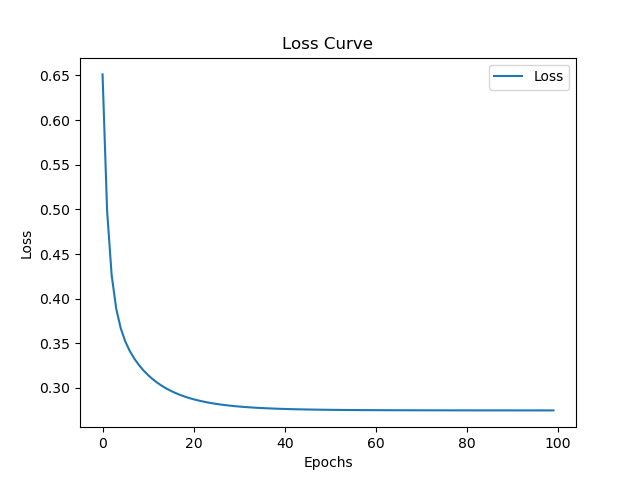
\includegraphics[width=0.3\textwidth]{LinearRegressionLoss1.png}}
    }
    \subfigure[Perceptron]{
    \adjustbox{valign=c}{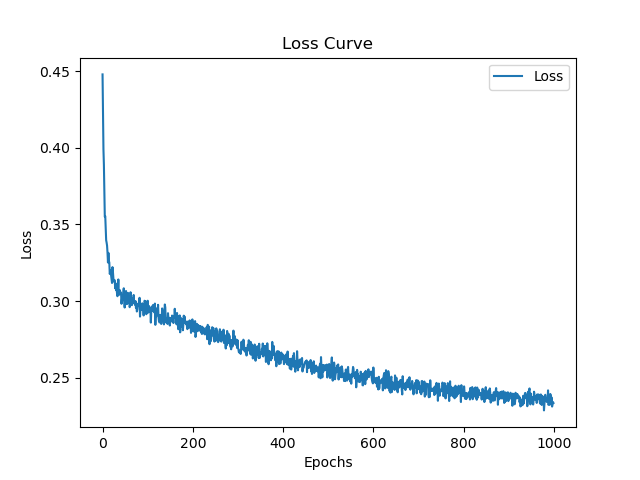
\includegraphics[width=0.3\textwidth]{PerceptronLoss1.png}}
    }
    \subfigure[Logistic Regression]{
    \adjustbox{valign=c}{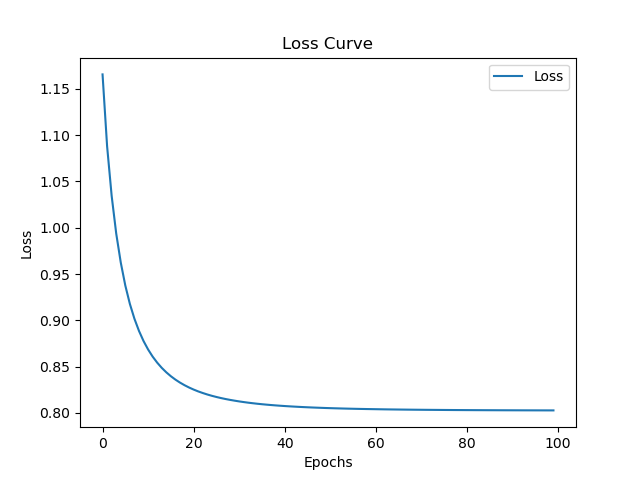
\includegraphics[width=0.3\textwidth]{LogisticRegressionLoss1.png}}
    }
    \subfigure[Linear Regression]{    
    \adjustbox{valign=c}{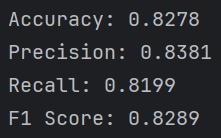
\includegraphics[width=0.25\textwidth]{LinearRegressionMetrics1.png}}
    }
    \hspace{5mm}
    \subfigure[Perceptron]{
    \adjustbox{valign=c}{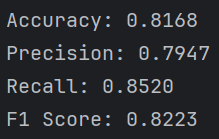
\includegraphics[width=0.25\textwidth]{PerceptronMetrics1.png}}
    }
    \hspace{5mm}
    \subfigure[Logistic Regression]{
    \adjustbox{valign=c}{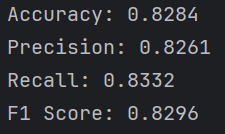
\includegraphics[width=0.25\textwidth]{LogisticRegressionMetrics1.png}}
    }
    \caption{Peformance of Linear Regression, Perceptron and Logistic Regression Models}
    \label{Figure 1}
\end{figure}

Dynamic learning rate can sometimes avoid oscillating and result in better
performance (See Figure~\ref{Figure 5} in \nameref{section:A}). However, if the primary
learning rate is already low enough, such method can slow down the training.

For the above 3 models, the performance of perceptron model seems a little bit worse than
the other two. However, generally, they get nearly the same scores in metrics. When it
comes to the speed of convergence, linear regression is the fastest, while perceptron is
the lowest. \\

MLP model has the best performance in classification. No matter how the hyperparameters
changes, the metrics can always be larger than $0.9$. Now we try to compare the
influence of the activation function on the performance. Figure~\ref{Figure 2} is the result
(MBGD, batch size=32, epochs=1000, learning rate=0.01, 2 hidden layers with 8 neorons in each).
Here we can see as for the training speed, ReLU is the fastest while sigmoid is the lowest,
and tanh is of the medium.

Also, deeper networks or more neurons in each layers is helpful to handel complex
datasets, while slow down the trianing speed. Figure~\ref{Figure 3} shows such
phenomenon (MBGD, batch size=32, epochs=1000, learning rate=0.01). In the image
captions, numbers in round brackets indicates the layer size.

\begin{figure}[H]
    \centering
    \subfigure[sigmoid]{    
    \adjustbox{valign=c}{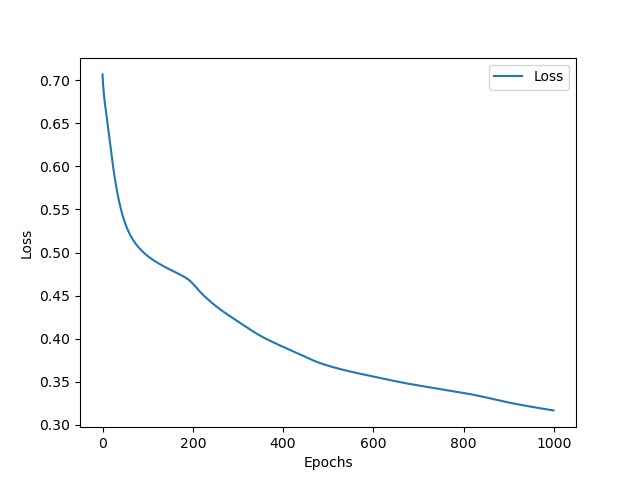
\includegraphics[width=0.3\textwidth]{mlpLoss1.png}}
    }
    \subfigure[tanh]{
    \adjustbox{valign=c}{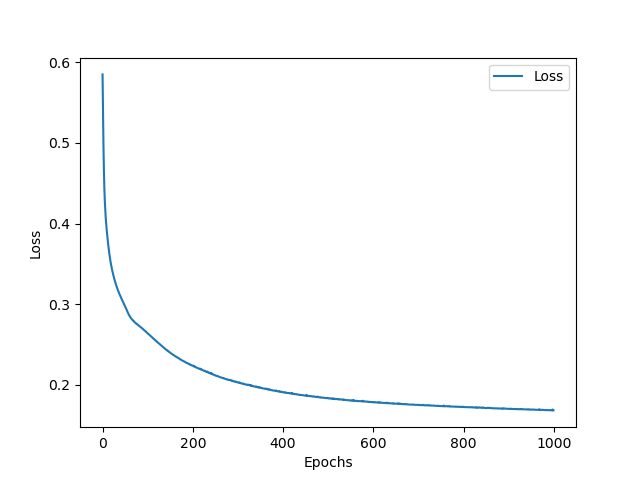
\includegraphics[width=0.3\textwidth]{mlpLoss2.png}}
    }
    \subfigure[ReLU]{
    \adjustbox{valign=c}{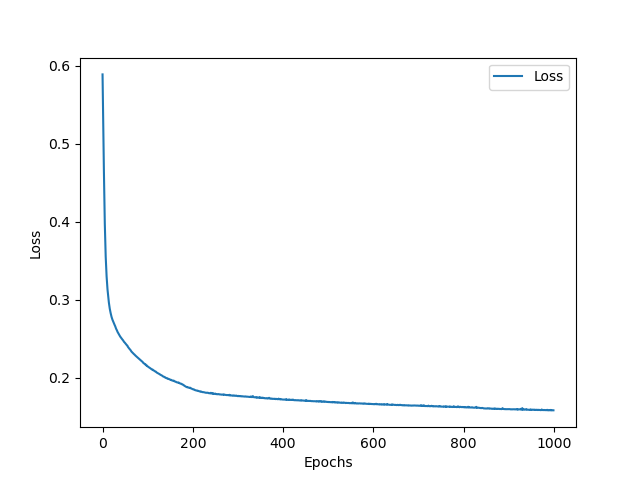
\includegraphics[width=0.3\textwidth]{mlpLoss3.png}}
    }
    \subfigure[sigmoid]{    
    \adjustbox{valign=c}{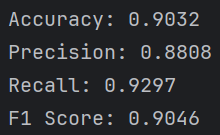
\includegraphics[width=0.25\textwidth]{mlpMetrics1.png}}
    }
    \hspace{5mm}
    \subfigure[tanh]{
    \adjustbox{valign=c}{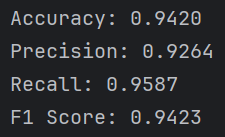
\includegraphics[width=0.25\textwidth]{mlpMetrics2.png}}
    }
    \hspace{5mm}
    \subfigure[ReLU]{
    \adjustbox{valign=c}{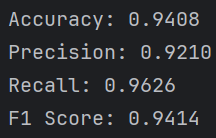
\includegraphics[width=0.25\textwidth]{mlpMetrics3.png}}
    }
    \caption{Influence of Different Activation Functions on MLP}
    \label{Figure 2}
\end{figure}

\begin{figure}[H]
    \centering
    \subfigure[(6,8,1)]{    
    \adjustbox{valign=c}{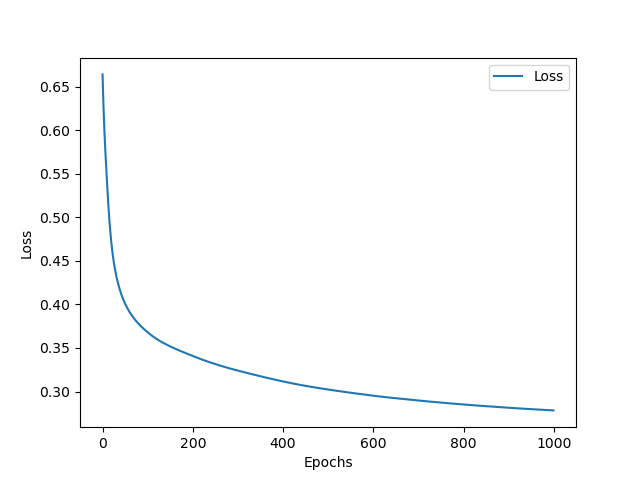
\includegraphics[width=0.3\textwidth]{mlpLoss4.png}}
    }
    \subfigure[(6,8,8,8,1)]{
    \adjustbox{valign=c}{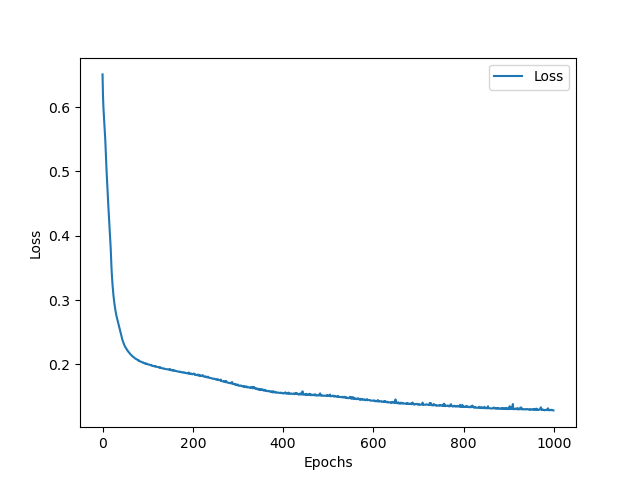
\includegraphics[width=0.3\textwidth]{mlpLoss5.png}}
    }
    \subfigure[(6,128,1)]{
    \adjustbox{valign=c}{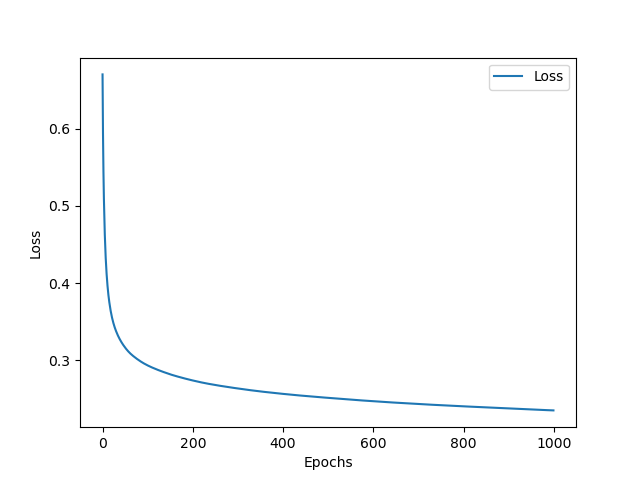
\includegraphics[width=0.3\textwidth]{mlpLoss6.png}}
    }
    \subfigure[(6,8,1)]{    
    \adjustbox{valign=c}{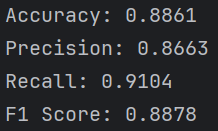
\includegraphics[width=0.25\textwidth]{mlpMetrics4.png}}
    }
    \hspace{5mm}
    \subfigure[(6,8,8,8,1)]{
    \adjustbox{valign=c}{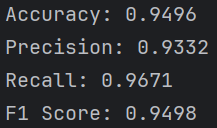
\includegraphics[width=0.25\textwidth]{mlpMetrics5.png}}
    }
    \hspace{5mm}
    \subfigure[(6,128,1)]{
    \adjustbox{valign=c}{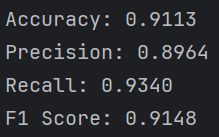
\includegraphics[width=0.25\textwidth]{mlpMetrics6.png}}
    }
    \caption{Influence of Different Size of Layers on MLP}
    \label{Figure 3}
\end{figure}

Standardization have positive effect on linear regression, logistic regression and MLP
models because it can accelerates the training. However, it has negtive effects on
perceptron, since we need to apply a smaller learning rate to avoid oscillating, and
the training becomes difficult (See Figure~\ref{Figure 6} in \nameref{section:A}).

\section{Conclusion}
The main difficulty to handle this dataset is that the samples labeled with 0 far more
than that labeled with 1, which causes the imbalance of data distribution. In such
condition, common training steps is not effective to make the model predict the
machine failure properly, since the model often tends to favor the majority class.
Oversampling provides more balanced training data, and weighted loss ensures the model
prioritizes the minority class during the training. Both of them improve the model's
performance.

Before applying oversampling and weighted loss, linear regression model performs the
worst, and alway gets 0 scores in precision, recall and F1-scores. Logistic regression and
MLP models have the highest scores, while still not perfect (see Figure~\ref{Figure 4} in \nameref{section:A}). 
It seems that perceptron, logistic
regression and MLP model born with the ability to handle binary classification, while
linear regression model is not suitable for such problems.

After applying oversampling and weightedloss, linear regression, perceptron and 
logistic regression models have nearly the same performance on predicting machine 
failure, with metrics above $0.8$ (Figure~\ref{Figure 1}). MLP model, still, performs the best amoung the
4 supervised learning models, with metrics above $0.9$ (Figure~\ref{Figure 2} and Figure~\ref{Figure 3}).

Now we can draw a conclusion for the performance on binary classification using the
4 supervised learning models:
\begin{enumerate}
    \item \textbf{Linear Regression Model}: Easy to implement, fast to train and
    predict, while unsuitable for binary classification directly.
    \item \textbf{Perceptron Model}: Easy to implement, while may not converge if the data
    is not linearly separable.
    \item \textbf{Logistic Regression Model}: It provides probabilistic output, and can
    handle som degree of non-linear data. Also, because of the linear boundary, the
    performance on complex non-linear problems is limited.
    \item \textbf{MLP Model}: It can handle complex, non-linear decision boundaries with
    multiple hidden layers. When it comes to the weaknesses, the training can be slow,
    and it requres careful tuning of many hyperparameters.
\end{enumerate} 

\section{Appendix}
\label{section:A}

Figure~\ref{Figure 4} shows the performances of the 4 models befor applying oversampling
and weighted loss, in contrast to Figure~\ref{Figure 1}, \ref{Figure 2} and \ref{Figure 3}:

\begin{figure}[H]
    \centering
    \subfigure[Linear Regression]{    
    \adjustbox{valign=c}{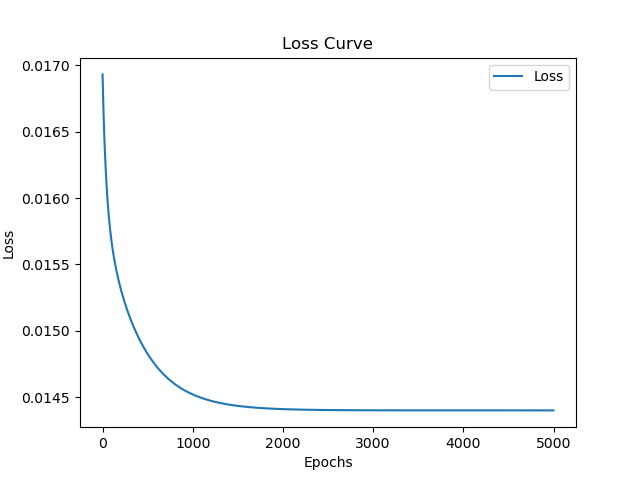
\includegraphics[width=0.22\textwidth]{LinearRegressionLoss2.png}}
    }
    \subfigure[Perceptron]{
    \adjustbox{valign=c}{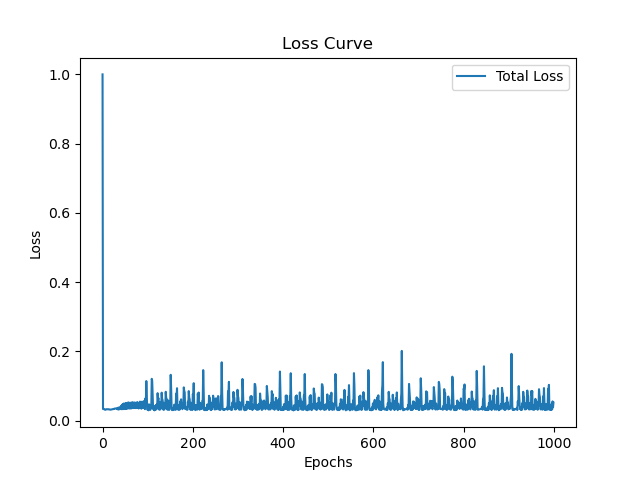
\includegraphics[width=0.22\textwidth]{PerceptronLoss2.png}}
    }
    \subfigure[Logistic Regression]{
    \adjustbox{valign=c}{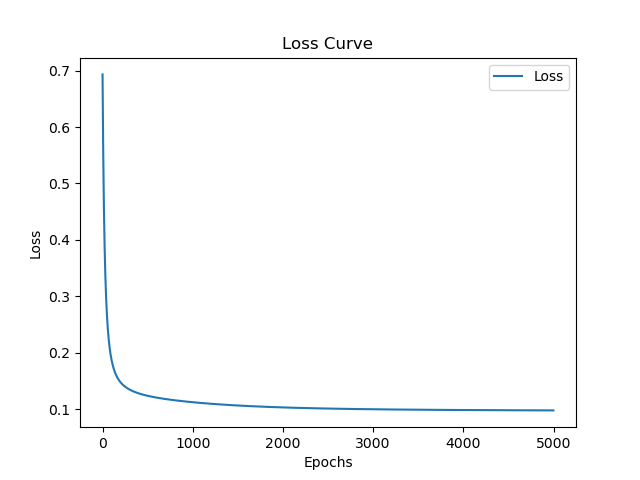
\includegraphics[width=0.22\textwidth]{LogisticRegressionLoss2.png}}
    }
    \subfigure[MLP]{
    \adjustbox{valign=c}{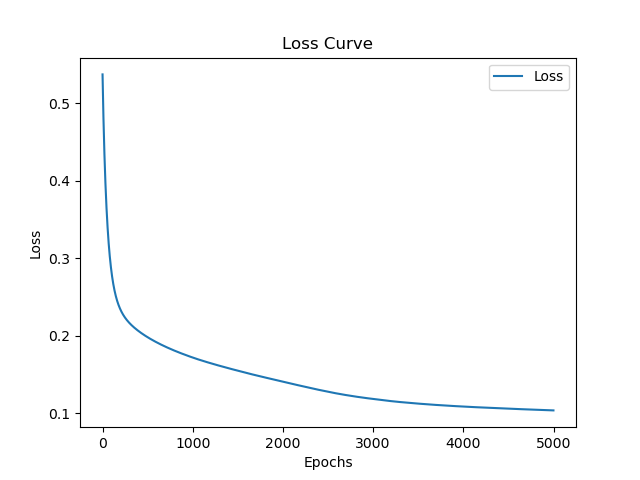
\includegraphics[width=0.22\textwidth]{MLPLoss7.png}}
    }
    \subfigure[Linear Regression]{    
    \adjustbox{valign=c}{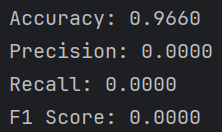
\includegraphics[width=0.2\textwidth]{LinearRegressionMetrics2.png}}
    }
    \hspace{2mm}
    \subfigure[Perceptron]{
    \adjustbox{valign=c}{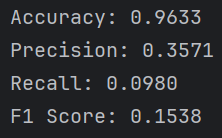
\includegraphics[width=0.2\textwidth]{PerceptronMetrics2.png}}
    }
    \hspace{2mm}
    \subfigure[Logistic Regression]{
    \adjustbox{valign=c}{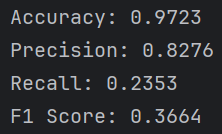
\includegraphics[width=0.2\textwidth]{LogisticRegressionMetrics2.png}}
    }
    \hspace{2mm}
    \subfigure[MLP]{
    \adjustbox{valign=c}{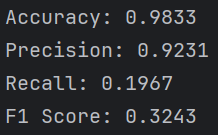
\includegraphics[width=0.2\textwidth]{MLPMetrics7.png}}
    }
    \caption{Peformance of Four Models Before Applying Oversampling and Weighted Loss}
    \label{Figure 4}
\end{figure}

Figure~\ref{Figure 5} shows the effects of applying dynamic learning rate. Here we
use linear regression model as an example, whose batch size $=32$, primary learning rate $=0.01$,
learning rate decay factor $=0.1$.

\begin{figure}[H]
    \centering
    \subfigure[Apply]{    
    \adjustbox{valign=c}{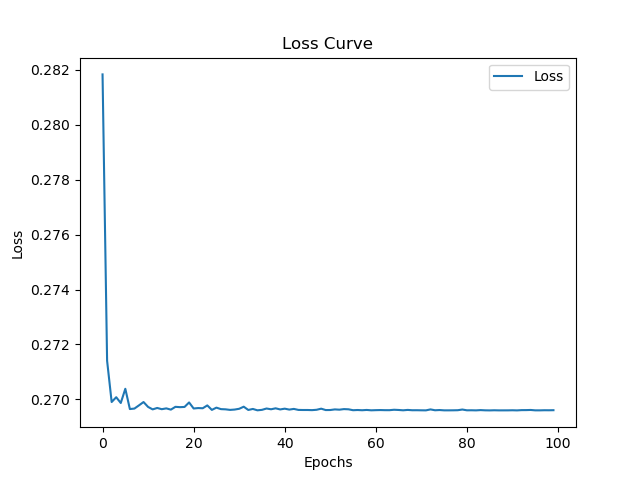
\includegraphics[width=0.35\textwidth]{DecayLoss1.png}}
    }
    \hspace{8mm}
    \subfigure[Not Apply]{
    \adjustbox{valign=c}{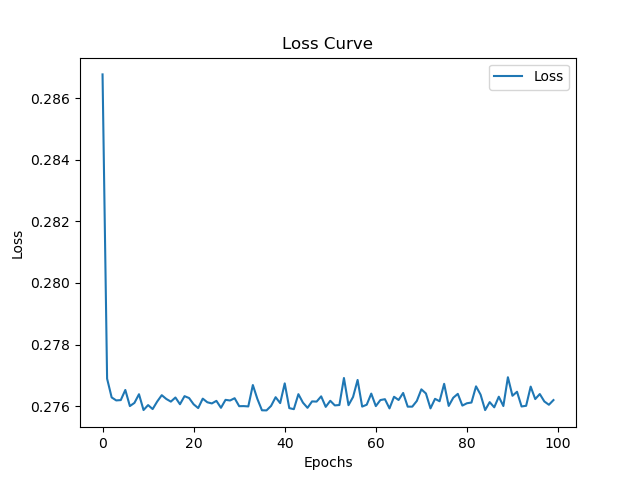
\includegraphics[width=0.35\textwidth]{DecayLoss2.png}}
    }
    \subfigure[Apply]{    
    \adjustbox{valign=c}{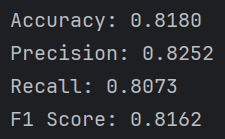
\includegraphics[width=0.25\textwidth]{DecayM1.png}}
    }
    \hspace{22mm}
    \subfigure[Not Apply]{
    \adjustbox{valign=c}{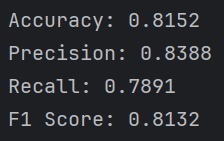
\includegraphics[width=0.25\textwidth]{DecayM2.png}}
    }
    \caption{The Effects of Applying Dynamic Learning Rate}
    \label{Figure 5}
\end{figure}

Figure~\ref{Figure 6} shows the perceptron model using standardization. It has
negative effect on training, in contrast to Figure~\ref{Figure 1}. Here we use
MBGD update, and batch size equal to $64$. Learning rate needs to be small to
prevent oscillating.

\begin{figure}[H]
    \centering
    \subfigure[lr=1e-8]{    
    \adjustbox{valign=c}{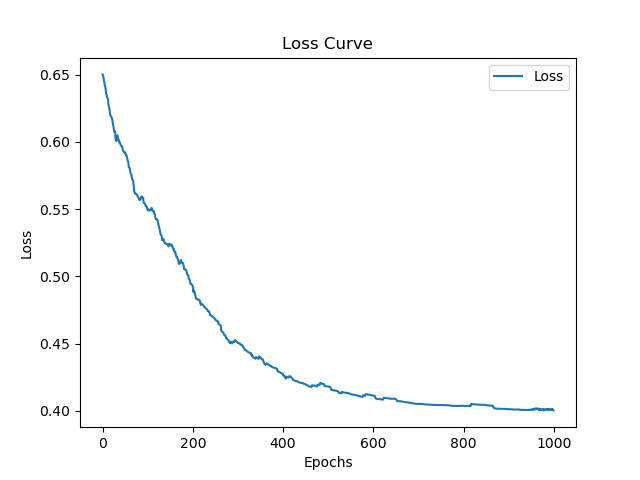
\includegraphics[width=0.35\textwidth]{PL1.png}}
    }
    \hspace{8mm}
    \subfigure[lr=1e-6]{
    \adjustbox{valign=c}{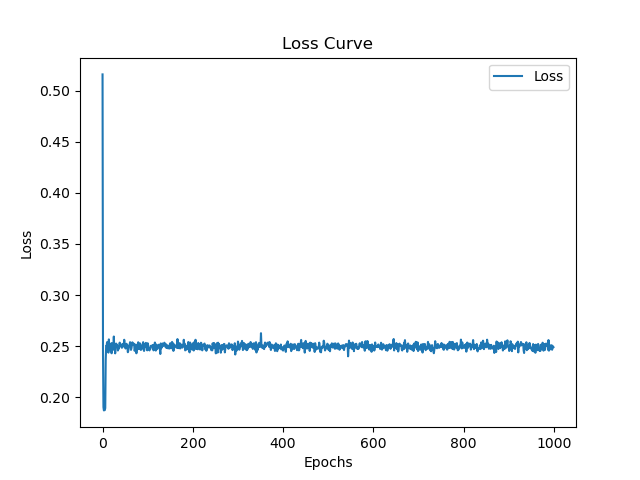
\includegraphics[width=0.35\textwidth]{PL2.png}}
    }
    \subfigure[lr=1e-8]{    
    \adjustbox{valign=c}{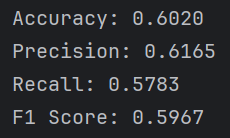
\includegraphics[width=0.25\textwidth]{PM1.png}}
    }
    \hspace{22mm}
    \subfigure[lr=1e-6]{
    \adjustbox{valign=c}{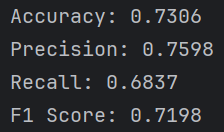
\includegraphics[width=0.25\textwidth]{PM2.png}}
    }
    \caption{Peceptron Using Standardization}
    \label{Figure 6}
\end{figure}

Figure~\ref{Figure 7} shows the effects of different hyperparameters on
linear regression. Larger batch size make loss curve smooth. Tiny learning
rate slow down the training, while larger one may cause oscillation.
The effects on logistic regression is the same.

\begin{figure}[H]
    \centering
    \subfigure[batch size=32, lr=0.01]{    
    \adjustbox{valign=c}{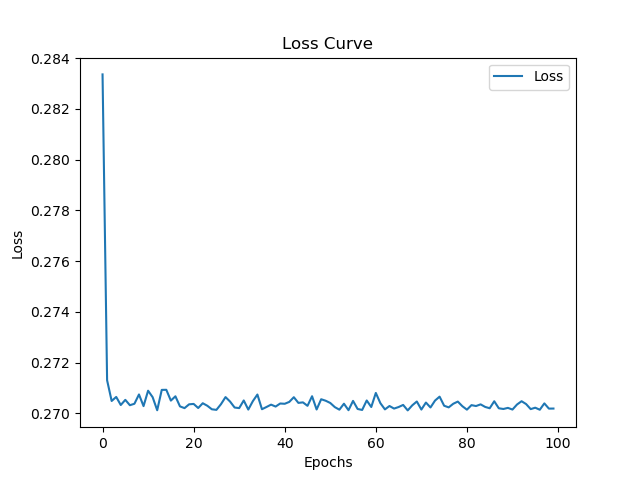
\includegraphics[width=0.3\textwidth]{LRL1.png}}
    }
    \subfigure[batch size=128, lr=0.01]{
    \adjustbox{valign=c}{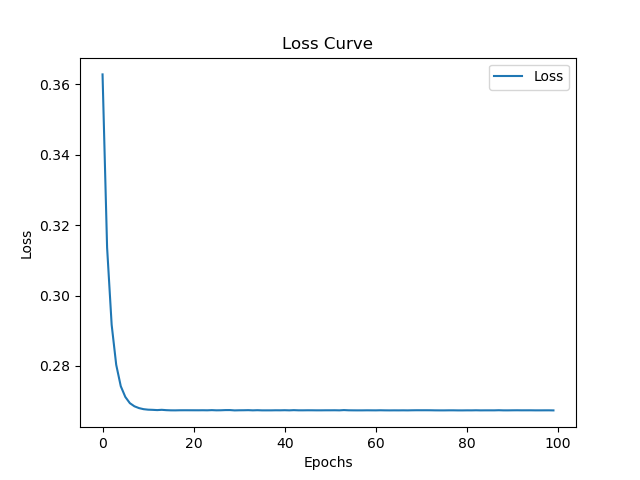
\includegraphics[width=0.3\textwidth]{LRL2.png}}
    }
    \subfigure[batch size=128, lr=0.001]{
    \adjustbox{valign=c}{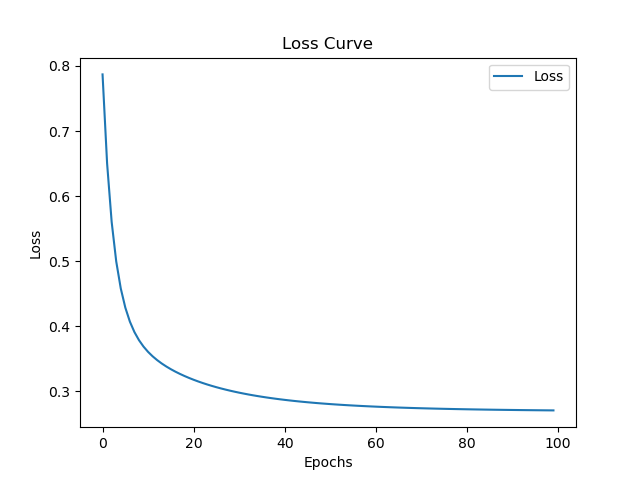
\includegraphics[width=0.3\textwidth]{LRL3.png}}
    }
    \subfigure[batch size=32, lr=0.01]{    
    \adjustbox{valign=c}{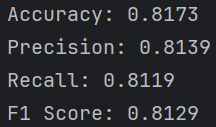
\includegraphics[width=0.25\textwidth]{LRM1.png}}
    }
    \hspace{7mm}
    \subfigure[batch size=128, lr=0.01]{
    \adjustbox{valign=c}{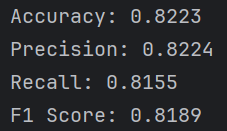
\includegraphics[width=0.25\textwidth]{LRM2.png}}
    }
    \hspace{7mm}
    \subfigure[batch size=128, lr=0.001]{
    \adjustbox{valign=c}{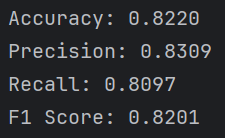
\includegraphics[width=0.25\textwidth]{LRM3.png}}
    }
    \caption{Linear Regression Model with Different Hyperparameters}
    \label{Figure 7}
\end{figure}



\end{document}